\section{Theorie}
\label{sec:Theorie}
Wenn sich Ladungen bewegen, erzeugen sie Magnetfelder. Die magnetische Flussdichte
dieses Magnetfeldes ist definiert als

\begin{equation}
    \label{eq:BmuH}
    \vec{B}=μ\vec{H},
\end{equation}
mit der \textbf{magnetischen Feldstärke $\vec{H}$} und der \textbf{Permeabilität $μ$}.
Die Permeabilität setzt sich dabei aus der Vakuum-Permeabilität $μ_0$ und der relativen
Permeabilität $μ_r$ zusammen.
\begin{equation}
    μ = μ_0μ_r\,.
\end{equation}
Fließt nun Strom durch einen Leiter, so besitzt dieser aufgrund der bewegten Elektronen
ein Magnetfeld, dessen Stärke sich durch das Biot-Savart-Gesetz bestimmen lässt.
Dabei gilt im Abstand $r$ mit dem durch den Leiter fließenden Stroms $I$
\begin{equation}
    \label{eq:biot-savart}
    \text{d}\vec{B}= \dfrac{μ_0 I}{4π} \dfrac{\text{d}\vec{s} \times \vec{r}}{r^3}\,.
\end{equation}\\

Wird der Leiter zu einem Ring mit Radius $R$ und Windungszahl $N$ gebogen, ergibt sich
aus \eqref{eq:biot-savart} die Gleichung
\begin{equation}
    \vec{B}(x) = N\dfrac{μ_0I}{2}\dfrac{R^2}{(R^2+x^2)^{3/2}} \vec{e}_x
\end{equation}
für die Magnetfeldstärke im Abstand $x$ vom Ringzentrum.\\

Bei einer langgestrecken Spule der Länge $l$ und dem Durchmesser $D$, $l>>D$, ist das Feld im
Inneren homogen und es gilt
\begin{equation}
    B=μ\dfrac{N}{L}I\,.
    \label{LangB}
\end{equation} 

Für einen Torus mit Radius $r_T<<l$ ist das äußere Magnetfeld null, lediglich im Inneren
existiert ein homogenes Magnetfeld mit
\begin{equation}
    B=μ\dfrac{N}{2πr_T}I\,.
    \label{RingB}
\end{equation}

Zwei gleichsinnig stromdurchflossene Kreisspulen mit Radius $R$ im Abstand $d=R$ werden
Helmholtz-Spulenpaar genannt, ihr Magnetfeld ergibt sich als Superposition der beiden
Einzelfelder der Spulen zu
\begin{equation}
    B(0)=μ_0N\dfrac{R^2}{(R^2+x^2)^{3/2}}I\,.
    \label{eq:HelmholtzB}
\end{equation}
Das Feld ist auf der Symmetrieachse, entlang dieser sich der Feldgradient zu
\begin{equation}
    \dfrac{\text{d}B}{\text{d}x} = -3μ_0R^2I\dfrac{x}{(R^2+x^2)^{3/2}}
\end{equation} ergibt.

Bei ferromagntischen Materialien findet sich auch ohne äußeres Magnetfeld ein \textbf{magnetisches Moment $\vec{M}$}. Sind diese \textbf{magnetischen Momente} in bestimmten Bereichen parallel zueinander ausgerichtet, wird
von Weiß'schen Bezirken gesprochen. Ein äußeres Magnetfeld führt zur Vergrößerung der Weiß'schen Bezirke, sorgt also dafür, dass sich die \textbf{magnetischen Momente} den äußeren Feldlinien entsprechend ausrichten.\\

Aufgrund der hohen relativen Permeabilität $μ_r$ ferromagntischer Stoffe besteht nicht länger ein linearer Zusammenhang zwischen $\vec{B}$ und $\vec{H}$, wie er in \eqref{eq:BmuH} beschrieben ist.
Dieser Magnetfeldverlauf lässt sich in einer Hysteresekurve in Äbhängigkeit vom äußeren Magnetfeld bzw. dem fließenden Strom darstellen. So ist zunächst $B(H=0)=0$. Wird nun ein äußeres Magnetfeld angelegt, steigt die Magnetisierung
auf Sättigungswert $B_s$ an. Diesen Anstieg nennt man \textit{Neukurve}. Bei Anlegen eines Gegenfeldes kehrt sich die Magnetisierung um. Auch ohne äußeres Feld bleibt jetzt eine Restmagnetisierung zurück, die \textit{Remanenz}.
Diese Remanenz kann durch ein \textit{Koerzitivkraft $H_c$} genanntes Gegenfeld wieder aufgehoben werden.
Wird das Gegenfeld weiter erhöht, wird auch die Magnetisierung negativ, bis sie den Sättigungswert $-B_s$ erreicht. Eine erneute Umkehr des äußeren Feldes sorgt nun für die Entstehung eine dritten Kurve,
die erneut bis zum Sättigungswert $B_s$ läuft.\\
 
Insgesamt ensteht so eine ursprungsymmetrische Kurve, die \textit{Hysteresekurve}, hier in \autoref{fig:Hystereseschema} dargestellt.

\begin{figure}[H]
    \centering
    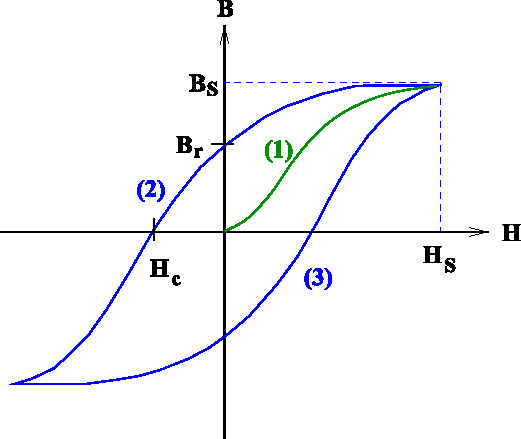
\includegraphics{Hystereseschema.pdf}
    \caption{Schematische Darstellung einer Hysteresekurve\cite{ap03}.}
    \label{fig:Hystereseschema}
  \end{figure}



